\chapter{Method}
\label{chap:method}

In this chapter I first describe the core techniques that have been used.
It is then followed by a detailed explanation of the proposed solution.
Finally I give the implementation details and settings.

\section{Neural Radiance Fields}

The Neural Radiance Fields approach (\cite{mildenhall2020nerf}) lies directly in the heart of the proposed solutions.
The continuous 5D function $F : (p,v) \xrightarrow{} (c, \omega)$ is required to be achieved in order to solve the novel view synthesis problem.
Given the spatial location $p \in \mathbb{R}$ and the 2D viewing direction $(\theta, \phi)$ (or its equivalent 3D Cartesian representation $v \in \mathbb{R}$),
one has to obtain the RGB color value $c$ and the probability volume density $\omega$ at this exact point $p$ under the viewing direction $v$.
To obtain the image of the scene, one can take a pin-hole camera at position $p_0$ and cast rays to the scene: $p(z) = p_0 + z\cdot v$.
The final visible color value $C(p,v)$ can then be evaluated using volume rendering approach \cite{niemeyer2020differentiable} along the ray $p$:
\begin{equation}
    C(p,v) = \int_{0}^{\infty} \omega(p(z)) \cdot c(p(z),v) dz
    \label{eq:rendering_equation}
\end{equation}
, $\omega(p(z))$ is a probability weight function
\begin{equation}
    \omega(p(z)) = \tau_c(p(z)) \sigma(p(z))
\end{equation}
, where $\tau_c(p(z)) = e^{\int_0^z \sigma(p(s)) ds}$ denotes the accumulated transmittance along the ray up to the point $p(z)$, $\sigma(p(z))$ is the volume density at point $p(z)$ and the probability property is held: $\int_0^\infty \omega(p(z))dz = 1$

\begin{figure}[t]
    \centering
    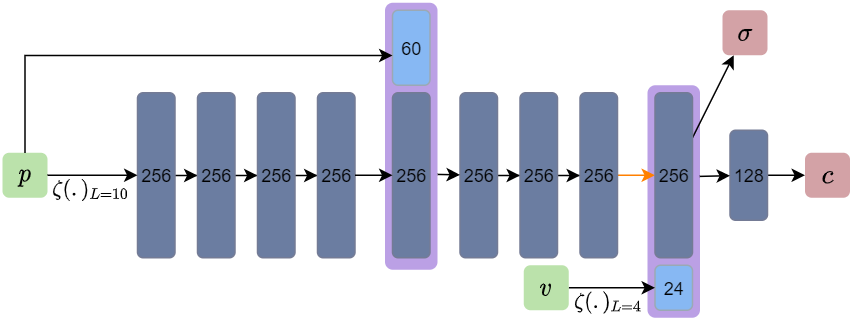
\includegraphics[width=0.6\textwidth]{figures/mlp_nerf.png}
    \caption{MLP used in NeRF \cite{mildenhall2020nerf} Dark blue boxes represent hidden layers. Black arrows indicate FC-layers with sigmoid activation, orange arrows - FC-layers without activation. $\zeta(.)$ stays for positional encoding function. $\sigma$ is 1D volume density, $c$ is a 3D color value. }
    \label{fig:mlp_nerf}
\end{figure}

\im{This paragraph should probably be moved to the related work.. somehow}
\cite{mildenhall2020nerf} propose to use a Multi-Layer Perceptron (MLP) as a representation
of an implicit function $F = F_\Theta$ with parameters $\Theta$.
The scheme structure of original NeRF's MLP is outlined in \Cref{fig:mlp_nerf}.
The position $p(z)$ is first encoded using position encoding function $\zeta(\cdot)$ (positional encoding is described in section \ref{subsec:pos_enc}) and then is processed with 8 fully-connected neural layers with ReLU activations.
The resulting feature vector is then concatenated with positionally encoded vector direction $v$
before the the volume density $\sigma(p(z))$ and the color value $c(p(z), v)$ is outputed.
The important concept here is that $\sigma$ only depends on point $p(z)$
whilst the color value $c$ is view dependant as well.
This setting is required to encourage the MLP to be multi-view consistent.

In order to perform the volume rendering, the continuous integral from equation \Cref{eq:rendering_equation} has to be solved.
One can estimate this integral using a discrete set of densely sampled points as proposed by \cite{mildenhall2020nerf}.
Separating each ray into $N$ bins and drawing random samples from each bin
makes the representation able to learn continuous function
while only using finite number of samples.
The estimate for the integral $C(p, v)$ will have a form (\cite{mildenhall2020nerf}, \cite{max1995optical}):

\begin{equation}
    C(p, v) \approx \sum_{i=1}^{N} \tau_c(p_i) (1 - e^{-\sigma(p_i) \delta_i}) c(p_i, v)
\end{equation}

, where $p_i = p(z_i)$ for brevity, $\tau_c(p_i) = e^{-\sum_{j=0}^i \sigma(p_j) \delta_j }$ is the accumulated transmittance and $\delta_i = z_{i+1} - z_i$ is the distance between adjacent sample points.

\subsection{Positional encoding}
\label{subsec:pos_enc}

Neural networks are known as a highly representative class of functions (\cite{hornik1989multilayer}).
However, recent works (\cite{rahaman2019spectral}, \cite{tancik2020fourfeat}) demonstrate the tendency of
biasing towards low frequency functions during training of deep neural networks.
The results can be smoothed and blurry as frequency-dependant learning speed
is much slower for high-frequency parts of the scene.
\cite{rahaman2019spectral} show that one can highly improve the quality of the MLP outputs
by using an embedding, which maps inputs to a higher dimensional space before passing them to the MLP.

The positional encoding function $\zeta(p) : \mathbb{R} \xrightarrow{} \mathbb{R}^{2L}$ as proposed by \cite{mildenhall2020nerf}, \cite{vaswani2017attention} is represented by Fourier series in the following form:

\begin{equation}
    \zeta(p) = (\sin(2^0\pi p), \cos(2^0\pi p), ..., \sin(2^{L-1}\pi p), \cos(2^{L-1}\pi p))
\end{equation}



\section{Implicit Neural Reflectance Field}

Existing BRDF models limits the type of scenes that can be captured
and successfully reconstructed afterwards.
To model object appearance one can employ neural network, which is able to get trained for a very complex appearance representations.
In this work I \im{we?} call this technique as "Implicit scheme".

Texture predictor not only is dependant on view direction,
but also requires the light direction and distance to light source
(for modelling the light attenuation effect).
Figure \# shows the network structure for this approach.

\begin{enumerate}
    \item Light rays are not sampled (-> varying light transmittance either not considered or assumed to get learned by network\im{???})
    \item |--> Tangential space for coordinates (and parametrization as half-vectors. not done)
\end{enumerate}

Since the appearance effects happen mostly in a local coordinate frame, the usage of the global direction vectors implies on the model to learn global to local coordinate system transformation. Although this is generally achievable, the overall complexity of the task can be too overwhelming for the model and some kind of correlations might affect the model. In order to increase the training performance this transformation can be done deterministically and the view and light directions in local coordinate frame are to be passed to the input of the model.

The usage of the cartesian vectors is not very effective for reflectance representations. The half diff vectors (rusinkiewicz parametrization) can be used instead of positionally encoded l and v.
\sm{or in combination with positional encoding}




\section{Explicit Neural Reflectance Field \im{for arbitrary light source}}

The NRF inherits very poor performance behavior from NeRF,
which limits it to only be feasible for the co-located light source setting.
However, with some optimization techniques \cite{NSVF, ...} can be used to make this method practical.

Using Octree with Sparse Voxels \cite{NSVF} highly increases the efficiency of sampling view rays,
and using voxel features allows to use smaller networks,
which also speeds up the training.

This efficiency improvement makes the general problem statement with an arbitrary light source feasible.


\section{In-Voxel Approximation}

Using the octree allows to approximate light rays sampling inside voxels in order to increase the performance of the method.

Instead of performing inverse CDF sampling as it is done for view rays, one can do the following:
\begin{enumerate}
    \item Bravely \sm{colloquial} assume the media homogenious inside voxels and boldly approximate it as constant
    \item Under the same brave assumption perform some sampling inside the voxel once at N iterations (e.g. right after pruning has been performed)
    \item The in-voxel sampling can be lighter than inverse CDF (e.g. just sample the center of voxel, or voxel corners + trilinear interpolation)
\end{enumerate}


% NSVF proposed a good technique of using Sparse Voxel Trees in order to increase the rendering speed. However, the scene is still lacking the light interaction.

% One can achieve this by also passing light directions along with distance to the light source into the network, in order to make it distinguish different surface properties for different view and light directions.








% This is some test area for new mathematical helper macros to nicely visualize mathematical formulas.

% \section{Numbers}
% \begin{align}
%     \mathbb{C}
%     \qquad
%     \mathbb{R}
%     \qquad
%     \mathbb{Q}
%     \qquad
%     \mathbb{Z}
%     \qquad
%     \mathbb{N}
% \end{align}

% \section{Numbers with physical units}
% \begin{align}
%     \SI{1.23}{\meter\per\second}
% \end{align}
% \begin{align}
%     \si{\meter\per\second}
% \end{align}
% \begin{align}
%     \SI{1.23\pm0.45}{\meter\per\second}
% \end{align}
% \begin{align}
%     \SI{3e8}{\meter\per\second}
% \end{align}
% \begin{align}
%     \SI{32}{\giga\byte} = \SI{32e9}{\byte}
% \end{align}
% \begin{align}
%     \SI{32}{\gibi\byte} = \SI[exponent-base=2]{32e30}{\byte}
% \end{align}

% \section{Norm, Dot, Abs, Interval}
% \begin{align}
%     \pi = \const
% \end{align}
% \begin{align}
%     1 \in \interval{0}{2}
% \end{align}
% \begin{align}
%     1 \in \order{n}
% \end{align}
% \begin{align}
%     \evalat{ \frac{\partial f}{\partial x} }{ x = 0 }
% \end{align}
% \begin{align}
%     \norm{p} \qquad \norm{\frac{p}{2}}
% \end{align}
% \begin{align}
%     \abs{p} \qquad \abs{\frac{p}{2}}
% \end{align}
% \begin{align}
%     \dotproduct{p}{q} \qquad \dotproduct{\frac{p}{2}}{q}
% \end{align}
% \begin{align}
%     \crossproduct{p}{q} \qquad \crossproduct{\frac{p}{2}}{q}
% \end{align}

% \section{Vector, Matrix}
% \begin{align}
%     \vec{p} \qquad \vecarrow{p}
% \end{align}
% \begin{align}
%     \vec{p}^{\transposed}
% \end{align}
% \begin{align}
%     \gradient{\vec{p}}
% \end{align}
% \begin{align}
%     \divergence{\mat{A}}
% \end{align}
% \begin{align}
%     \laplacian{\mat{A}}
% \end{align}
% \begin{align}
%     \mat{A}
% \end{align}
% \begin{align}
%     \set{K} , K
%     \qquad
%     \set{N} , N
% \end{align}
% \begin{align}
%     \neighborhood{\vec{p}} = \left\{ \vec{q} \mid \norm{\vec{p} - \vec{q}} < \epsilon \right\}
% \end{align}

% \section{Set operations}
% \begin{align}
%     A \intersect B
% \end{align}
% \begin{align}
%     A \union B
% \end{align}
% \begin{align}
%     A \difference B
% \end{align}

% \section{Derivative, Integral, Sum, Probability}
% \begin{align}
%     \int_H x \, dx
% \end{align}
% \begin{align}
%     \sum_H x
% \end{align}
% \begin{align}
%     \probability{x}
% \end{align}
% \begin{align}
%     \probabilitygiven{x}{y}
% \end{align}
% \begin{align}
%     \expectation{x}
% \end{align}
% \begin{align}
%     \deviation{x}
% \end{align}
% \begin{align}
%     \variance{x}
% \end{align}


% \section{Lemma, Theorem, Corollary}
% \begin{lemma}
%     This is a lemma.
% \end{lemma}
% \begin{proof}
%     Proof of lemma.
% \end{proof}

% \begin{theorem}
%     This is a theorem.
% \end{theorem}
% \begin{proof}
%     Proof of theorem.
% \end{proof}

% \begin{corollary}
%     This is a corollary.
% \end{corollary}
% \begin{proof}
%     Proof of corollary.
% \end{proof}


